\documentclass[11pt]{article}
\usepackage[T1,T2A]{fontenc}
\usepackage[utf8]{inputenc}
\usepackage[english,russian]{babel}
\usepackage{graphicx}
\usepackage{amsmath}
\graphicspath {{img/}}
\title{\textbf{Лабораторная работа №5\\
<<Исследование устройств фазового преобразования сигналов в системах передачи информации>>}}
\author{Матяш А.А., ККСО-01-19}
\date{}
\addtolength{\topmargin}{-3cm}
\addtolength{\textheight}{3cm}
\begin{document}
\maketitle
\thispagestyle{empty}
\textbf{Цель работы:} ознакомление с устройством, работой фазовых модуляторов демодуляторов сигналов и приобретение практических навыков и моделирования этих устройств. 
\section{Перечень элементов на схемах}
\subsection{<<Схема исследования ФМ сигналов>>}
\begin{itemize}
    \item[-] Четырех канальный осциллограф
    \item[-] Источник переменного тока (1 В, 10 кГц, 0$^{\circ}$)
    \item[-] Спектральный анализатор
    \item[-] Генератор сигналов
    \item[-] Множитель напряжения (1 В/В, 0 В)
\end{itemize}
\subsection{<<Схема частотного модулятора и демодулятора>>}
\begin{itemize}
    \item[-] Четырех канальный осциллограф
    \item[-] Резистор (100 Ом)
    \item[-] Конденсатор (0.5 мкФ)
    \item[-] Генератор сигналов
    \item[-] Источник переменного тока (1 В, 10 кГц, 0$^{\circ}$)
    \item[-] Множитель напряжения (1 В/В, 0 В) 2 шт.
\end{itemize}
\subsection{<<Схема системы передачи информации с фазовой манипуляцией>>}
\begin{itemize}
    \item[-] Генератор слов 
    \item[-] Четырех канальный осциллограф
    \item[-] ЦАП
    \item[-] Источник постоянного тока (20 В)
    \item[-] Источник постоянного тока (5 В)
    \item[-] Источник переменного тока (1 В, 10 кГц, 0$^{\circ}$)
    \item[-] Множитель напряжения (1 В/В, 0 В) 2 шт.
    \item[-] Резистор (100 Ом) 3 шт.
    \item[-] Линия связи без потерь (100 Ом, 1 нс)
    \item[-] Конденсатор (0.3 мкФ)
    \item[-] Гистерезис по напряжению (0 В 1 В/В)
    \item[-] Логический анализатор 
\end{itemize}
\section{Копии окон схемных файлов с позиционными
обозначениями}
\subsection{<<Схема исследования ФМ сигналов>>}
\includegraphics[width=1\linewidth]{img/1/scheme.jpg} 
\subsection{<<Схема частотного модулятора и демодулятора>>}
\includegraphics[width=1\linewidth]{img/2/scheme.jpg} 
\subsection{<<Схема системы передачи информации с фазовой манипуляцией>>}
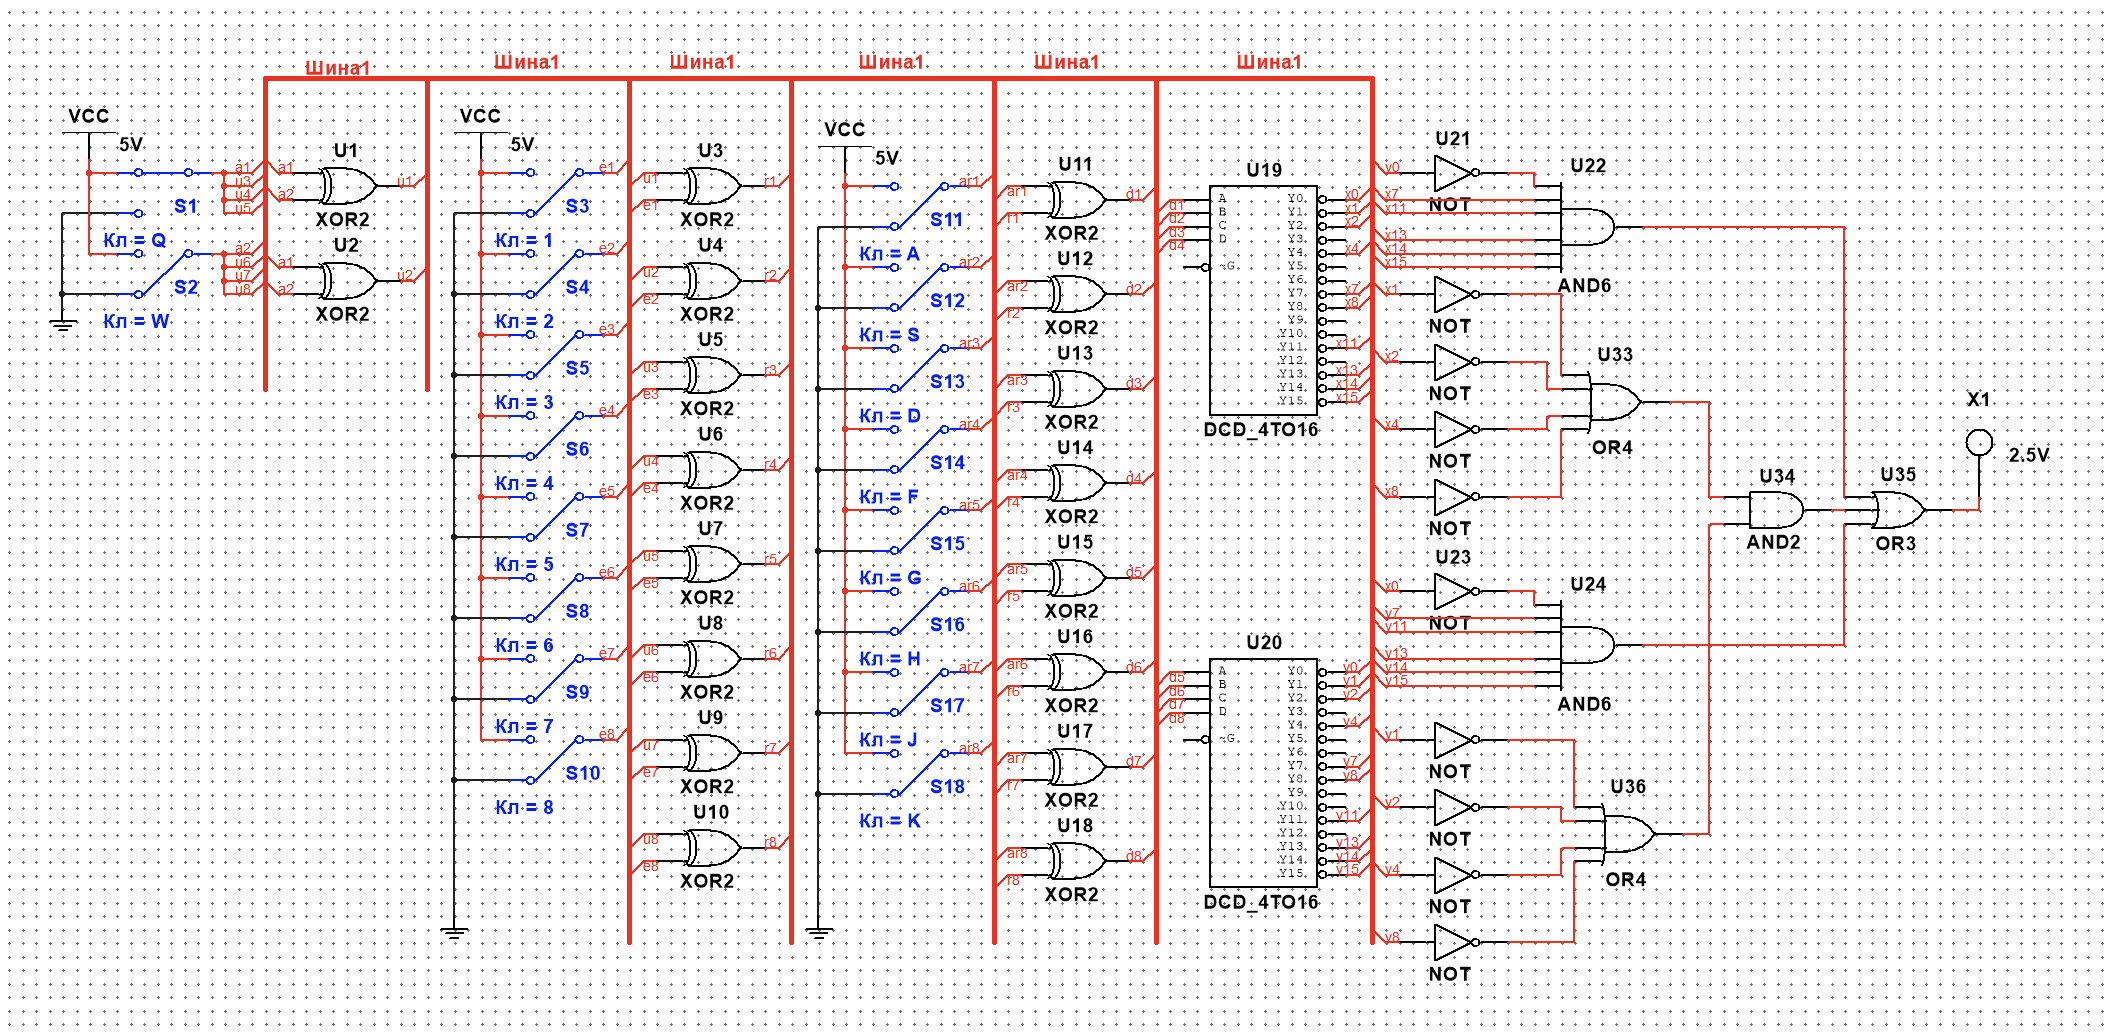
\includegraphics[width=1\linewidth]{img/3/scheme.png} 
\section{Результаты расчетов и измерений приборами}
\subsection{<<Схема исследования ФМ сигналов>>}
Осциллограмма:\\
\includegraphics[width=1\linewidth]{img/1/osc.jpg} 
Спектрограмма:\\
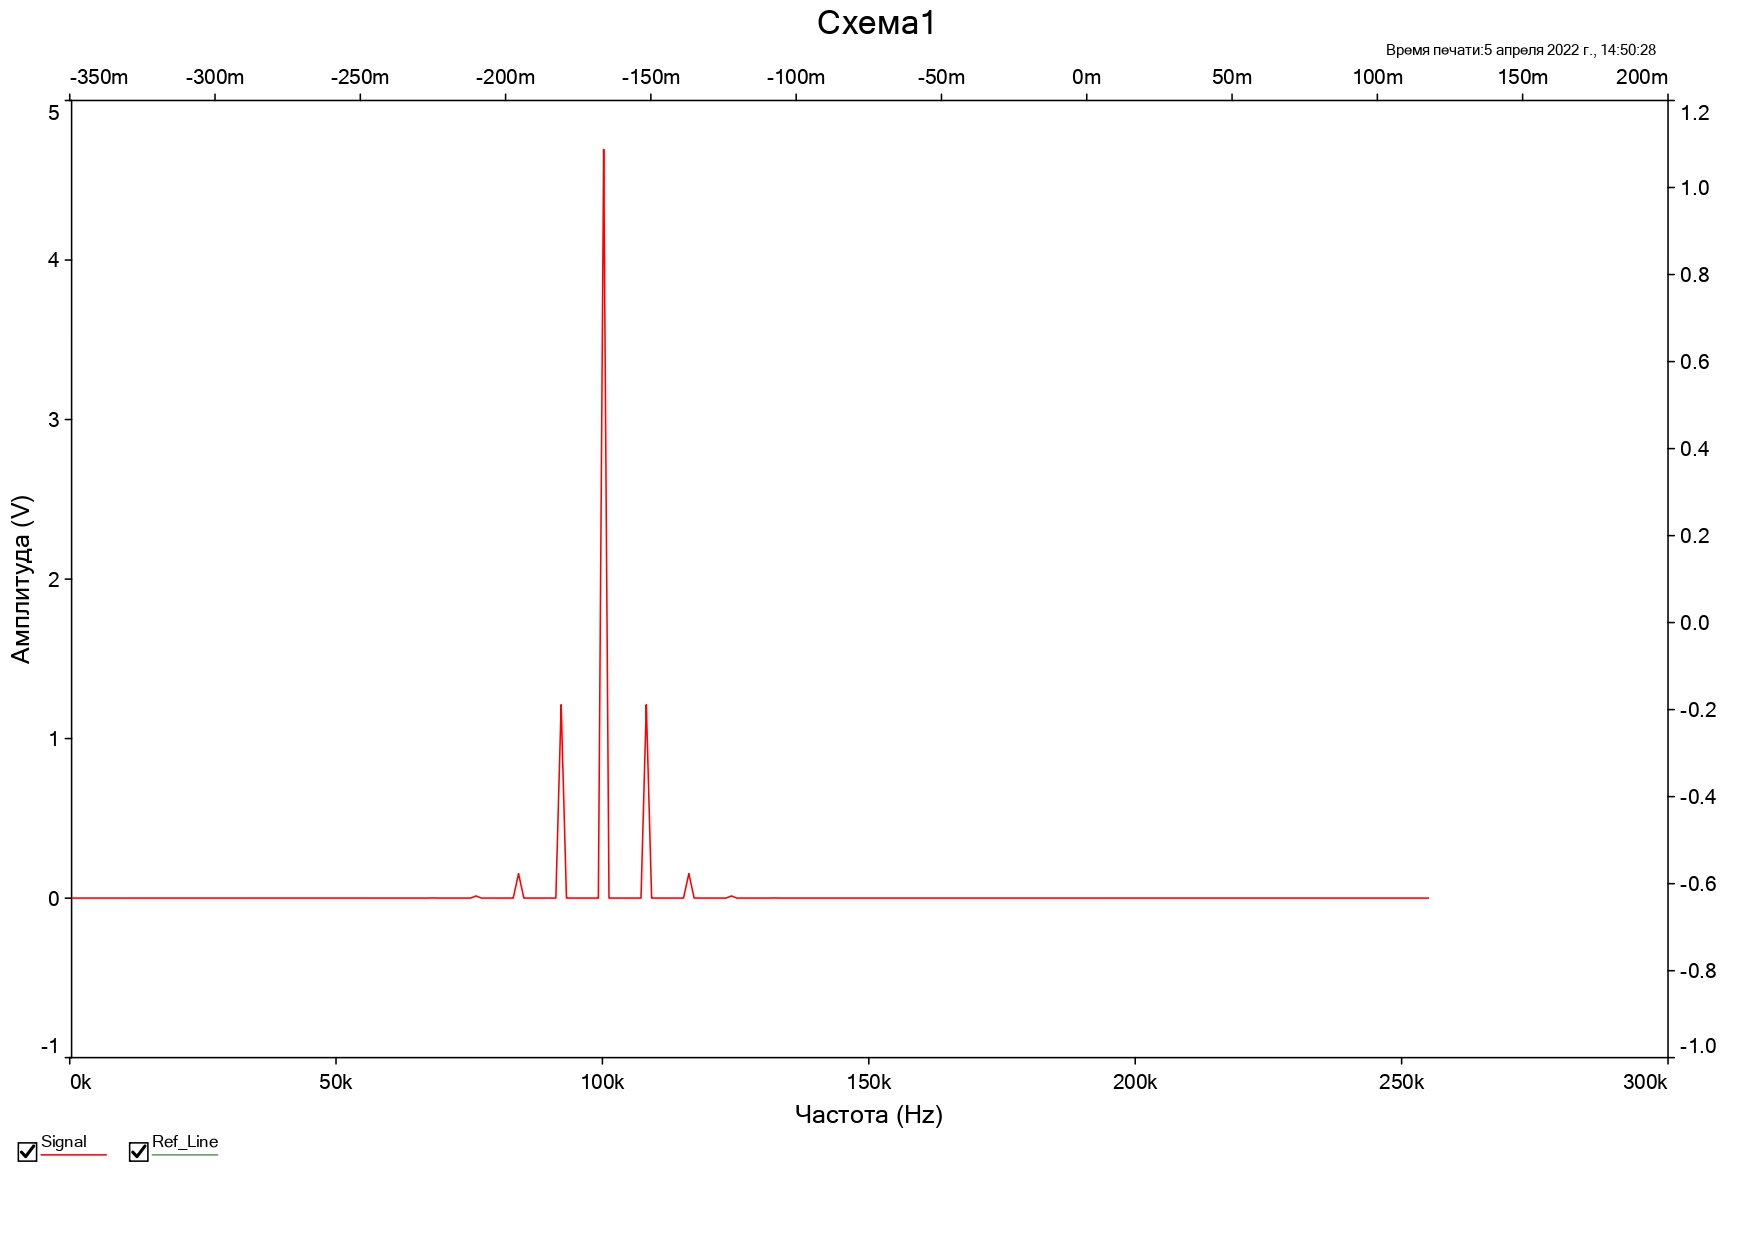
\includegraphics[width=1\linewidth]{img/1/specter.jpg}
\subsection{<<Схема частотного модулятора и демодулятора>>}
Осциллограмма:\\
\includegraphics[width=1\linewidth]{img/2/osc.jpg}
\subsection{<<Схема системы передачи информации с фазовой манипуляцией>>}
\begin{itemize}
\item Скорость 1 Кбит/c:\\
Осциллограмма:\\
\includegraphics[width=1\linewidth]{img/3/1kbs/osc.jpg}
Логический анализатор:\\
\includegraphics[width=1\linewidth]{img/3/1kbs/loganaliz.jpg}
\item Скорость 5 Кбит/c:\\
Осциллограмма:\\
\includegraphics[width=1\linewidth]{img/3/5kbs/osc.jpg}
Логический анализатор:\\
\includegraphics[width=1\linewidth]{img/3/5kbs/loganaliz.jpg}
\item Скорость 10 Кбит/c:\\
Осциллограмма:\\
\includegraphics[width=1\linewidth]{img/3/10kbs/osc.jpg}
Логический анализатор:\\
\includegraphics[width=1\linewidth]{img/3/10kbs/loganaliz.jpg}
\end{itemize}
\textbf{Вывод:} в ходе выполнения лабораторной работы мы изучили устройства фазового преобразования сигналов и их работу. Приобрели практические навыки, научились моделировать эти устройства.
\end{document}

